\documentclass[titlepage]{article}
\usepackage{babel}
\usepackage{amsmath}
\usepackage{amssymb}
\usepackage{amsthm}
\usepackage{stmaryrd} %ligtning

\usepackage{tabto} %tabulator mit \tab
\usepackage{tikz}
\usetikzlibrary{automata, arrows.meta, positioning, shadows, shapes.geometric} % automaten zeichnen
\usepackage[utf8]{inputenc}
\pagestyle{plain}
\pagenumbering{arabic}
\renewcommand{\arraystretch}{1.3} %vertikaler abstand von tabellen
\usepackage[left=20mm, right=15mm, top=25mm, bottom=7mm, paper=a4paper]{geometry}

\renewcommand{\contentsname}{Inhaltsverzeichnis}
\renewcommand{\]}{\right]}
\renewcommand{\[}{\left[}
\renewcommand{\)}{\right)}
\renewcommand{\(}{\left(}
\renewcommand{\|}{\;|\;}
\newcommand{\n}{\newline}
\renewcommand{\l}{\linebreak}



\begin{document}\begingroup\let\clearpage\relax
	%header
	\begin{center}
	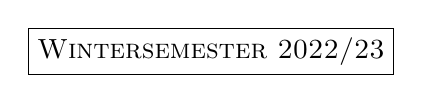
\begin{tikzpicture}
		\draw (0,0) node[draw, rectangle]{\textsc{Wintersemester 2022/23}};
	\end{tikzpicture}
	\hrulefill\\
	\begin{center}
		\LARGE\textsc{Automaten und Berechenbarkeit - Übung 04} \normalsize\\
	\end{center}
	\hrulefill
	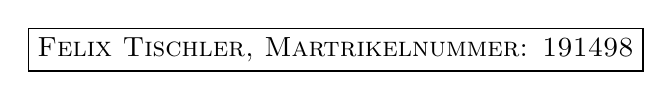
\begin{tikzpicture}
		\draw (0,0) node[draw, rectangle]{\textsc{Felix Tischler, Martrikelnummer: 191498}};
	\end{tikzpicture}
	\date{\today}
\end{center}
	
	%task one
	\section*{Aufgabe 1}
	Wir betrachten die Sprache $L=\{a^ib^jc^k\mid i,j,k\in\mathbb{N},i=0\;oder\;j=k\}$
		\paragraph{(a)} Geben Sie eine kontextfreie Grammatik an, die $L$ erzeugt.
		\paragraph{(b)} L ist nicht regulär. Begründen Sie, dass man durch direkte Anwendung des Pumping-\\Lemmas für reguläre Sprachen \textbf{nicht} zeigen kann, dass $L$ nicht regulär ist.
		\paragraph{(c)} Zeigen Sie, dass $L$ nicht regulär ist.
	\section*{Aufgabe 2}Gegeben sind die Sprachen $L=\{w\in\{0,1\}^*\mid\#_1(w)\equiv0\mod3\}$ und\\ $L_2=\{w\in\{0,1\}^*\mid w\text{ enthält das Teilwort 011 nicht}\}.$ \\Konstruieren Sie einen DFA $M$ mit $L(M)=\overline{L_1}\cap L_2$
	
	\section*{Aufgabe 3} Es sei $L=\{xuxvx\mid x\in\{a,b\}\land u,v\in\{a,b\}^*\land\mid u\mid=\mid v\mid\}$
		\paragraph{(a)} Zeigen Sie, dass $L$ nicht regulär ist.
		\paragraph{(b)} Geben Sie eine kontextfreie Grammatik an, die $L$ erzeugt.

\endgroup\end{document}